\documentclass[a4 paper]{article}
% Set target color model to RGB
\usepackage[inner=1.5cm,outer=1.5cm,top=2.5cm,bottom=2.5cm]{geometry}
\usepackage{setspace}
\usepackage[rgb]{xcolor}
\usepackage{verbatim}
\usepackage{amsgen,amsmath,amstext,amsbsy,amsopn,tikz,amssymb,tkz-linknodes}
\usepackage{fancyhdr}
\usepackage[colorlinks=true, urlcolor=blue,  linkcolor=blue, citecolor=blue]{hyperref}
\usepackage[colorinlistoftodos]{todonotes}
\usepackage{rotating}
\usepackage{enumitem}
\usepackage{amssymb}
\usepackage{tikz}
\usetikzlibrary{arrows}


%\usetikzlibrary{through,backgrounds}
\hypersetup{%
pdfauthor={Arman Shokrollahi},%
pdftitle={Homework},%
pdfkeywords={Tikz,latex,bootstrap,uncertaintes},%
pdfcreator={PDFLaTeX},%
pdfproducer={PDFLaTeX},%
}
%\usetikzlibrary{shadows}
\usepackage[francais]{babel}
\usepackage{booktabs}
\newcommand{\ra}[1]{\renewcommand{\arraystretch}{#1}}

      \newtheorem{thm}{Theorem}[section]
      \newtheorem{prop}[thm]{Proposition}
      \newtheorem{lem}[thm]{Lemma}
      \newtheorem{cor}[thm]{Corollary}
      \newtheorem{defn}[thm]{Definition}
      \newtheorem{rem}[thm]{Remark}
      \numberwithin{equation}{section}

\newcommand{\report}[5]{
   \pagestyle{myheadings}
   \thispagestyle{plain}
   \newpage
   \setcounter{page}{1}
   \noindent
   \begin{center}
   \framebox{
      \vbox{\vspace{2mm}
    \hbox to 6.50in { {\bf EC4213/ET5402/CT5303:~Machine learning and deep learning \hfill Fall 2019} }
       \vspace{4mm}
       \hbox to 6.28in { {\Large \hfill #1 \hfill}}
       \vspace{1mm}
       \hbox to 6.28in { {\hfill #2  \hfill} }
       \vspace{3mm}
       \hbox to 6.28in { {\it Instructor: #3 \hfill #4 (#5)}}
      \vspace{2mm}}
   }
   \end{center}
   \markboth{#5 -- #1}{#5 -- #1}
   \vspace*{4mm}
}

\newcommand{\bbF}{\mathbb{F}}
\newcommand{\bbX}{\mathbb{X}}
\newcommand{\bI}{\mathbf{I}}
\newcommand{\bX}{\mathbf{X}}
\newcommand{\bx}{\mathbf{x}}
\newcommand{\bY}{\mathbf{Y}}
\newcommand{\bw}{\mathbf{w}}
\newcommand{\bepsilon}{\boldsymbol{\epsilon}}
\newcommand{\balpha}{\boldsymbol{\alpha}}
\newcommand{\bbeta}{\boldsymbol{\beta}}
\newcommand{\0}{\mathbf{0}}
\DeclareMathOperator*{\argmax}{arg\,max}
\DeclareMathOperator*{\argmin}{arg\,min}
\newcommand\gldec[2]{
\underset{#1}{\overset{#2}{\gtrless}}
}
\usepackage{titlesec}
\titlespacing*{\section}
{1.5em}{1.5em}{1em}
\titlespacing*{\subsection}
{1.5em}{1em}{1em}


\begin{document}
\report{Report for CA1}{}{Jonghyun Choi}{Jwa Younkyung}{20165174}

REPORT1. why is this computation equivalent to computing classification accuracy? \\
    It is a good classification when the prediction value using X and the value of Y are identical. Since Y is -1 or 1, the Y value greater than 0 and the prediction value greater than 0 are compared and the average of the compared values is accuracy.

REPORT2. Please dicsuss the reason that the training accuracy tend to decrease. Also, discuss the reason that the test accuracy not monotonically increasing. \\

\begin{figure}[!htb]
    \center{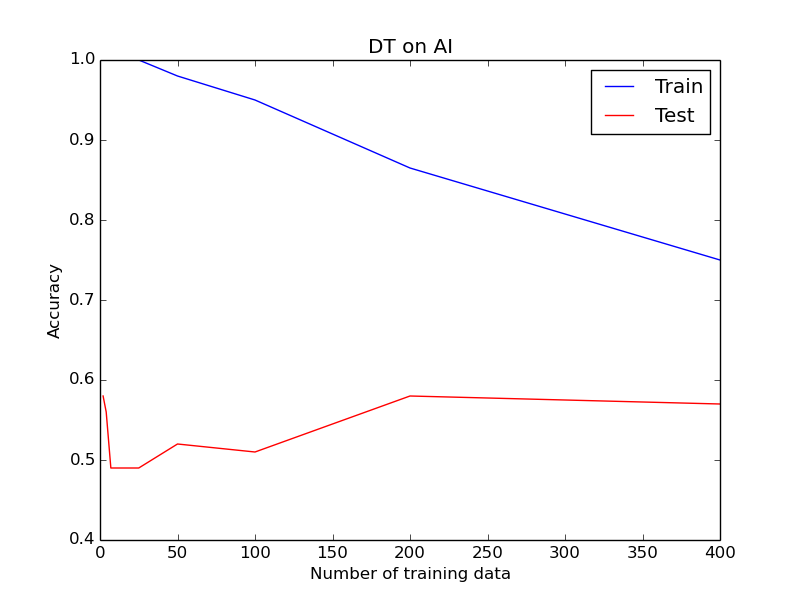
\includegraphics[width=0.4\textwidth]{./accuracy_numData.png}}
    \caption{DT on AI.}
    \label{fig:dataset}
\end{figure}

Large numbers of data drive more bias, which tends to decrease due to bias training accuracy. If the number of data used for training is very small and the test data has similar data to the training data, the accuracy can be larger than others. \\

REPORT3. If the implementation is correct, you will observe the training accuracy monotonically increasing and test accuracy tumbling. Please discuss the behavior of the training accuracy and test accuracy. \\

\begin{figure}[!htb]
    \center{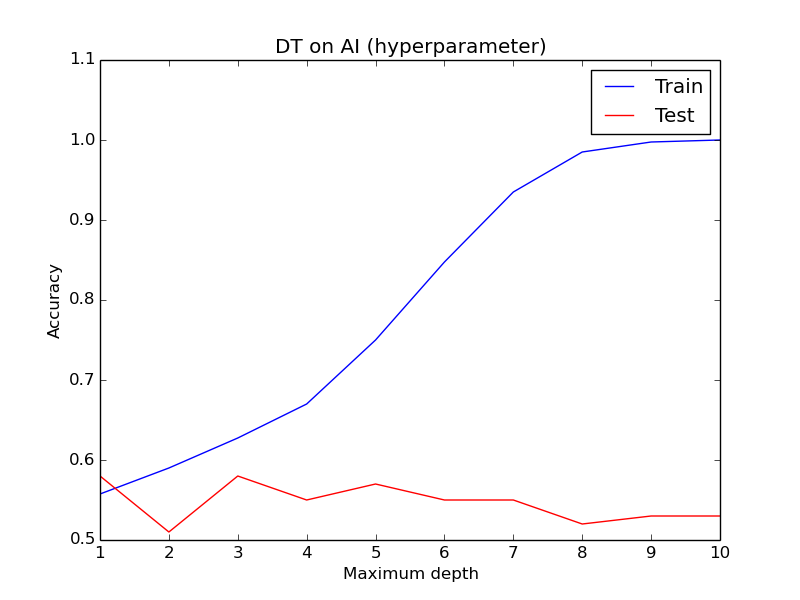
\includegraphics[width=0.4\textwidth]{./accuracy_maxDepth.png}}
    \caption{DT on AI(hyperparameter).}
    \label{fig:dataset}
\end{figure}

Increasing the maximum depth will overfit the model. Therefore, it is very suitable for training sets and improves the accuracy of training sets. As the variance of the model increases, the shape of the decision tree continues to change. As a result, the test set and model may or may not fit well. So accuracy is tumbling. \\

REPORT4. Train a decision tree on the CG dataset with a maximum depth of `3`. In the write-up, first, draw out the decision tree for this classifier (but put in the actual course names/ids as the features). Then, discuss about this tree: do these courses are indicative of whether someone might take CG?

Result of train data is: \\
 \newcommand\tab[1][1cm]{\hspace*{#1}}
Branch 6 \\
\tab Branch 34 \\
\tab[2cm] Branch 48 \\
\tab[3cm] Leaf -1.0 \\
\tab[3cm] Leaf 1.0 \\
\tab[2cm] Branch 27 \\
\tab[3cm] Leaf -1.0 \\
\tab[3cm] Leaf 1.0 \\
\tab Branch 54 \\
\tab[2cm] Branch 32 \\
\tab[3cm] Leaf -1.0 \\
\tab[3cm] Leaf 1.0 \\
\tab[2cm] Branch 53 \\
\tab[3cm] Leaf 1.0 \\
\tab[3cm] Leaf 1.0 \\

It may look like this : \\


\tikzset{
  treenode/.style = { align=center, inner sep=0pt, text centered,
    font=\sffamily},
  arn_n/.style = {treenode, rectangle, black, font=\sffamily\bfseries, draw=black,
    fill=white, text width=10em, text height=1em, text depth=5em},% arbre rouge noir, noeud noir
  arn_x/.style = {treenode, circle, draw=black,
    minimum width=2.0em, minimum height=1.5em}% arbre rouge noir, nil
}

\begin{tikzpicture}[
    ->,>=stealth',
    level/.style={sibling distance = 9cm/#1,
    level distance = 3cm,
  }] 
\node [arn_n] {132,\\object-oriented programming ii}
    child{ node [arn_n] {631,\\program analysis and understanding } 
            child{ node [arn_n] {733,\\computer processing of pictorial information } 
            	            child{ node [arn_x] {-1.0}} 
							child{ node [arn_x] {1.0}}
            }
            child{ node [arn_n] {434,\\introduction to human-computer interaction}
							child{ node [arn_x] {-1.0}}
							child{ node [arn_x] {1.0}}
            }
    }
    child{ node [arn_n] {773,\\computational linguistics ii }
            child{ node [arn_n] {460,\\computational methods } 
							child{ node [arn_x] {-1.0}}
							child{ node [arn_x] {1.0}}
            }
            child{ node [arn_n] {754,\\computational geometry }
							child{ node [arn_x] {1.0}}
							child{ node [arn_x] {1.0}}
            }
	}
; 
\end{tikzpicture} \\
This decision tree means that whether someone might take CG depends on whether or not "object-oriented programming ii", "program analysis and understanding", "computer processing of pictorial information", "introduction to human-computer interaction", "computational linguistics ii", "computational methods" and "computational geometry" are taken. Only 7 features are involved in TookCG.
\\

REPORT5. Compare the test accuracy before and after the pruning by plotting a comparative graph. And discuss the effect of pruning in terms of training accuracy, test accuracy and generalization performance. Also, discuss the good hyperparameter (eg., 0.05) for each dataset. \\
I fixed some code in runClassifier and ran the code as below for make curve \\
$>>>$curve = runClassifier.learningPrunedCurveSet(dt.DT({'maxDepth': 5}), datasets.CFTookAI) \\
$>>>$runClassifier.plotCurve('DT on AI with pruning', curve) \\
$>>>$curve = runClassifier.hyperparamPCurveSet(dt.DT({'maxDepth': 5}), 'maxPvalue', [0.01, 0.02, 0.03, 0.04, 0.05, 0.06, 0.07, 0.08, 0.09, 0.1], datasets.CFTookAI) \\
$>>>$runClassifier.plotCurve('DT on AI with pruning (hyperparameter)', curve) \\
$>>>$curve = runClassifier.comparativeTestingCurveSet(dt.DT({'maxDepth': 5}), datasets.CFTookAI) \\
$>>>$runClassifier.plotCurve('Comparative Test', curve) \\
$>>>$curve = runClassifier.comparativeTrainingCurveSet(dt.DT({'maxDepth': 5}), datasets.CFTookAI) \\
$>>>$runClassifier.plotCurve('Comparative Train', curve) \\

\begin{figure}[!htb]
    \center{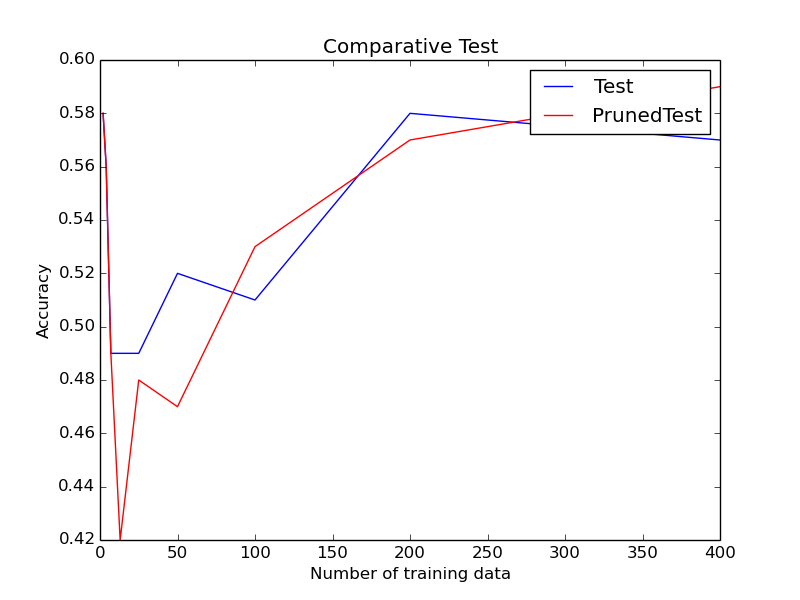
\includegraphics[width=0.4\textwidth]{./comparative_test.png}}
    \caption{Comparative Test.}
    \label{fig:dataset}
\end{figure}


\begin{figure}[!htb]
    \center{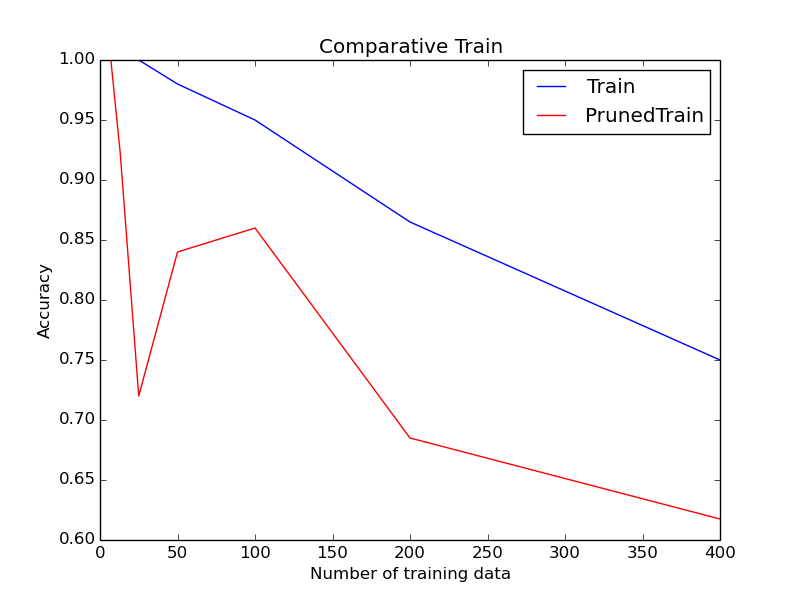
\includegraphics[width=0.4\textwidth]{./comparative_train.png}}
    \caption{Comparative Train.}
    \label{fig:dataset}
\end{figure}

Pruning decrease training accuracy and increases testing accuracy little by little. Therefore, pruning can make the model more general.

\begin{figure}[!htb]
    \center{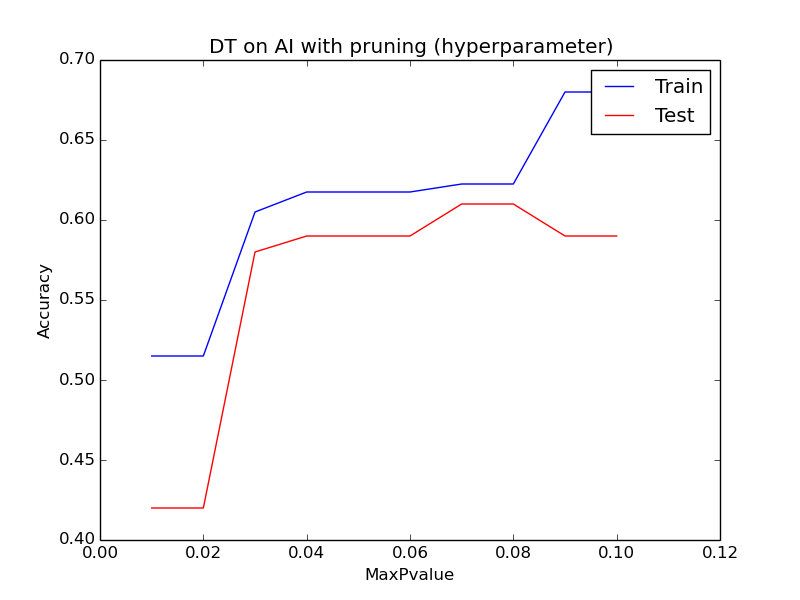
\includegraphics[width=0.4\textwidth]{./accuracy_maxPvalue.png}}
    \caption{DT on AI with pruning(hyperparameter).}
    \label{fig:dataset}
\end{figure}

In Fig.\ref{fig:dataset}, accuracy of test set is highest at about 0.08 maxPvalue. So, set maxPvalue = 0.08 is good for pruning.   

\end{document}





